%
% main.tex -- Paper zum Thema Machine Learning und Klimamodelle
%
% (c) 2018 Hochschule Rapperswil
%
\tikzstyle{inputNode}=[draw,circle,minimum size=10pt,inner sep=0pt]
\tikzstyle{stateTransition}=[-stealth, thick]

\chapter{Machine Learning und Klimamodelle\label{chapter:learning}}
\lhead{Machine Learning und Klimamodelle}
\begin{refsection}
\chapterauthor{Martin Stypinski}
	
	

Wettervorhersagen basieren auf Modellen, welche eine Näherung der Realität darstellen. Diese Modelle versuchen mit einer beschränkten Parameter Anzahl die Natur möglichst gut zu abstrahieren. Je nach Anwendung liegt der Schwerpunkt der Modelle auf einer Genauigkeit über grosse Gebiete (Klimaforschung) oder auf einer hohen Genauigkeit in kleinen Regionen (lokaler Wetterdienst). Vor einigen Jahren haben Grover et al. \cite{Groover:2015} versucht mittels neuronaler Netzwerke eine Wettervorhersage zu tätigen.

Neuronale Netzwerke sind ein Teil der Forschung im Bereich des maschinellen Lernens (Machine Learning). Machine Learning als Domäne geht zurück bis in die frühen 60er Jahre und hatte den Ursprung in Mustererkennungsforschung und computergestützter Lerntheorie. Die konstante Geschwindigkeitssteigerung der Hardwarebranche bescherte dieser rechenintensiven Domäne einen neuen Frühling. Was vor 10 Jahren noch den Welt stärksten Supercomputer beanspruchte, kann heute auf einem einzelnen starken Server in gleicher Zeit berechnet werden. Dieser extreme Leistungsschub der vergangenen Jahrzehnte ermöglich heute viele Probleme auf dem heimischen PC zu lösen, welche vor 10 Jahren noch ganze Rechenzentren beansprucht haben.

Im Gegensatz zur Wettervorhersage mit entwickelten Modellen ist es mittels künstlicher neuronaler Netzwerke (KNN) möglich ein Blackbox zu trainieren und später zu verwenden. Die Parameter erlernt das System selbst und kann anhand dieser gelernter Parameter eine Vorhersage treffen. Mit einer grosszügigen Datengrundlage ist das System im Stande viel bessere Lösungen zu approximieren als mit einfacheren Modellen möglich ist. Allein dieser Umstand ist ein treibender Faktor um anspruchsvolle Probleme mittels diser Methode zu lösen. Mit einer grossen Datengrundlage kann das System sehr gute Lösungen approximieren, dies kommt der Wettervorschung zu gute, da eine grosse Menge an Daten verfügbar ist.

Für die Forschung sind grosse Modelle sehr interessant um aber ein tieferes Verständnis für die Funktionsweise von neuronalen Netzwerken zu erlangen, wurde hier entschieden sich auf sehr kleine Modelle zu konzentrieren, diese dafür aber sehr genau zu analysieren.

\section{Die Wärmeleitungsgleichung als diskretes ML Problem}
Die Wärmeleitungsgleichung (gem. Kapitel xyz) ist eine partielle Differential Gleichung welche für diesen Anwendungszweck in einer Dimension gemäss Gleichung \ref{eq:waermeleitung-1d} beschrieben werden kann.
\begin{equation}
\frac{\partial T}{\partial t} = \kappa \frac{\partial^2}{\partial x^2} T
\label{eq:waermeleitung-1d}
\end{equation}
Das gewählte Model soll eine Vorhersage über die Zeit machen können. Sowohl die Zeit als auch der Ort wird diskretisiert und der Zeitschritt $T(x,y) \rightarrow T(x,t+1)$ erlernt. Die Lösung kann diskret approximiert werden. 

Um die diskrete Lösung herzuleiten wird das Modell eines Stabs $S$ (1D) genommen. Der Stab wird nun unterteilt in $N+2$ äquidistante Punkte (mit Abstand $h$), wobei am Anfang und am Ende des Stabes die Temperatur konstant ist. Es existieren folglich $S(x_0, \dots, x_{N+1})$ Punkte und folglich gilt $x_0 = a$, $x_{N+1} = b$. Die Lösung kann nun mittels Eulerverfahren bestimmt werden.
\begin{equation}
T(x,t+\Delta t) = T(x,t) + \Delta t \cdot  \frac{\partial T}{\partial t} = T(x,t) + \Delta t \cdot \kappa \frac{\partial^2}{\partial x^2} T
\end{equation}

Folglich werden die zweiten Ableitung $T_{xx}$ benötigt, welche hier symetrisch hergeleitet wurde:

\begin{align}
T_{x}(x, t)  &= \frac{T(x-\frac{1}{2}h, t) - T(x+\frac{1}{2}h, t)}{h}\\
T_{xx}(x, t) &= \frac{T_{x}(x-\frac{1}{2}h, t) - T_{x}(x+\frac{1}{2}h, t)}{h} \\
&= \frac{\frac{T(x-h, t) - T(x+h, t)}{h} - \frac{T(x, t) - T(x+1,t)}{h}}{h} = \frac{T(x-h, t) - 2 T(x, t) + T(x+h, t)}{h^{2}}
\end{align}

Aus der initialen Beziehung lässt sich nun folglich herleiten:

\begin{equation}
T(x,t) \rightarrow T(x,t+1) : T(x,t+1) = \frac{\kappa}{h^{2}} \Big( T(x-h,t) - 2 \cdot T(x,t) + T(x+h,t)  \Big)
\end{equation}

Dies lässt sich auch als Skalarprodukt für 3 Punkte des Stabes $S(x_0, \dots, x_{N+1})$ schreiben: 
\begin{equation}
T(x,t) \rightarrow T(x,t+1) : \begin{pmatrix} x_{k-1} & x_{k} & x_{k+1} \end{pmatrix} \cdot \underbrace{\frac{\kappa}{h^2} \begin{pmatrix} 1 \\ -2 \\ 1 \end{pmatrix}}_{\vec{w}} =  \frac{\kappa}{h^2} \cdot \left( 1 \cdot x_{k-1} - 2 \cdot x_{k} + 1 \cdot x_{k+1} \right)
\label{eq:sumvec}
\end{equation}
Der Vektor $\vec{w}$ in Gleichung \ref{eq:sumvec} hat die L1-Norm ($\|w\|_{1}:=\sum _{{i=1}}^{n}|w_{i}|$) von $1$. Dies ist zu begründen dadurch, dass keine Temperaturzunahme oder Temperaturabnahme im gesammten System über einen Zeitschritt stattfinden kann! Die Temperaturänderung geschieht lokal abhänig von der umliegenden Temperatur. Sie kann lokal wachsen oder fallen, nicht aber im gesammten System einen Trend entwickeln.

Es ist nun erklärt wie die Wärmeleitungsgleichung in einem 1 dimensionalen Stab mathematisch funktioniert. Dies Verfahren wird später verwendet um Trainingsdaten für ein neuronales Netzwerk zu erzeugen.


\subsection{Neuronales Netzwerk}

Um zu verstehen wie ein neuroneales Netzwerk für den 1 dimensionalen Stab entwickelt werden kann ist es wichtig zu verstehen wie ein neuronales Netzwerk funktioniert.

Das später verwendete künstliche neuronale Netzwerk (KNN) ist supervised. Supervised learning Methoden (vgl. Abbildung \ref{fig:mst_model_testing}) versuchen mittels Input $I_{t}$ und Output $O_{t}$ eine Abbildung $H$ zu finden, welche mit möglichst kleinem Fehler $I$ auf $O$ abbilden kann \cite{MIT:2015}. Dieser Schritt wird auch als Training bezeichnet. In einem zweiten Schritt der Prediction Phase wird versucht mittels der gelernten Abbildungsfunktion $H$ und neuen, unbekanntem Input $I_{p}$ einen Output $O_{p}$ vorherzusagen, ohne diesen bereits gekannt zu haben.

\begin{figure}
	\tikzstyle{decision} = [diamond, draw, fill=white, 
	text width=4.5em, text badly centered, node distance=3cm, inner sep=0pt]
	\tikzstyle{block} = [rectangle, draw, fill=white, 
	text width=5em, text centered, rounded corners, minimum height=4em]
	\tikzstyle{arrow} = [draw, -latex']
	\tikzstyle{cloud} = [draw, ellipse,fill=white, node distance=2.5cm, minimum height=2em, inner sep=-1pt]
	\begin{tabular}{cc}
		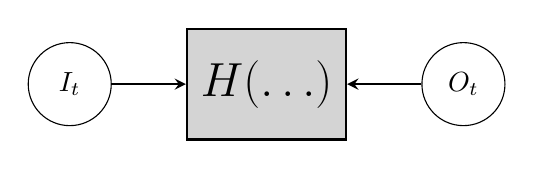
\begin{tikzpicture}
		\node[draw,thick,fill={rgb:black,1;white,5},minimum width=40pt,minimum height=40pt, inner sep=5pt] (H) at (0,0) {\LARGE $H(\dots)$};
		
		\node[inputNode,minimum size=30pt] (inp) at (-2.5, 0) {$I_{t}$};
		\node[inputNode,minimum size=30pt] (outp) at (2.5, 0) {$O_{t}$};
		\draw[stateTransition] (inp) to[out=0,in=180] node [midway, sloped, above] {} (H);
		\draw[stateTransition] (outp) to[out=180,in=0] node [midway, sloped, above] {} (H);
		\end{tikzpicture}
		&
		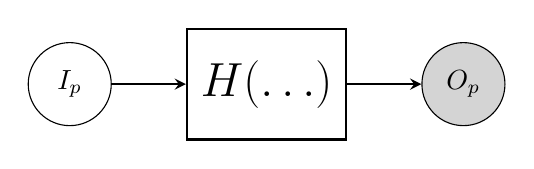
\begin{tikzpicture}
		\node[draw,thick,minimum width=40pt,minimum height=40pt, inner sep=5pt] (H) at (0,0) {\LARGE $H(\dots)$};
		
		\node[inputNode,minimum size=30pt] (inp) at (-2.5, 0) {$I_{p}$};
		\node[inputNode,fill={rgb:black,1;white,5}, minimum size=30pt] (outp) at (2.5, 0) {$O_{p}$};
		\draw[stateTransition] (inp) to[out=0,in=180] node [midway, sloped, above] {} (H);
		\draw[stateTransition] (H) to[out=0,in=180] node [midway, sloped, above] {} (outp);
		\end{tikzpicture}
	\end{tabular}
	
	\caption{\textbf{Links:} In der Trainingsphase wird die Abbildungsfunktion $H$ gelernt. \textbf{Rechts:} Die Predictionphase approximiert $O_{p}$ anhand der erlernten Funktion $H$.}
	\label{fig:mst_model_testing}
\end{figure}


Ein KNN besteht aus vielen einzelnen Neuronen die zusammen das Netzwerk bilden dies wird in Abbildung \ref{fig:mst_neuronalnetwork} verdeutlicht. Ein einzelnes Neuron ist eine gewichtete Summe mit Bias Parameter ($b$), zur Brechung der Linearität des Systems werden sogenante Aktivierungsfunktionen ($\sigma$) verwendet. Diese Funktion wird benötigt, damit das Netzwerk nicht eine linear Kombination von vielen Neuronen ist und somit vereinfacht zu einer einfachen Funktion werden kann. Die Neuronen werden in Gruppen angeordnet, welche oft als \textit{Input Layer}, \textit{Hidden Layer} und \textit{Output Layer} bezeichnet werden. 

\begin{figure}[h]
	\centering
	%\documentclass[crop, tikz]{standalone}
%\usepackage{tikz}



%\begin{document}
\begin{tikzpicture}
	\node[draw,circle,minimum size=25pt,inner sep=0pt] (x) at (0,0) {$\Sigma$ $\sigma$};

	\node[inputNode] (x0) at (-1, 2) {$\tiny +1$};
	\node[inputNode] (x1) at (-2, 0.75) {$\tiny x_0$};
	\node[inputNode] (x2) at (-2, 0) {$\tiny x_1$};
	\node[inputNode] (x3) at (-2, -0.75) {$\tiny x_2$};
	\node[inputNode] (xn) at (-2, -1.75) {$\tiny x_n$};

	\draw[stateTransition] (x0) to[out=0,in=90] node [midway, sloped, above] {$b$} (x);
	\draw[stateTransition] (x1) to[out=0,in=150] node [midway, sloped, above] {$w_0$} (x);
	\draw[stateTransition] (x2) to[out=0,in=180] node [midway, sloped, above] {$w_1$} (x);
	\draw[stateTransition] (x3) to[out=0,in=210] node [midway, sloped, above] {$w_2$} (x);
	\draw[stateTransition] (xn) to[out=0,in=240] node [midway, sloped, above] {$w_n$} (x);
	\draw[stateTransition] (x) -- (4,0) node [midway,above] {$\sigma \left(\sum\limits_{i=0}^{n}{w_ix_i}+b\right)$};
	\draw[dashed] (0,-0.43) -- (0,0.43);
	\node (dots) at (-2, -1.15) {$\vdots$};
	\node[inputNode, thick] (i1) at (6, 0.75) {};
	\node[inputNode, thick] (i2) at (6, 0) {};
	\node[inputNode, thick] (i3) at (6, -0.75) {};
	
	\node[inputNode, thick] (h1) at (8, 1.5) {};
	\node[inputNode, thick] (h2) at (8, 0.75) {};
	\node[inputNode, thick] (h3) at (8, 0) {};
	\node[inputNode, thick] (h4) at (8, -0.75) {};
	\node[inputNode, thick] (h5) at (8, -1.5) {};
	
	\node[inputNode, thick] (o1) at (10, 0.75) {};
	\node[inputNode, thick] (o2) at (10, -0.75) {};
	
	\draw[stateTransition] (5, 0.75) -- node[above] {$I_1$} (i1);
	\draw[stateTransition] (5, 0) -- node[above] {$I_2$} (i2);
	\draw[stateTransition] (5, -0.75) -- node[above] {$I_3$} (i3);
	
	\draw[stateTransition] (i1) -- (h1);
	\draw[stateTransition] (i1) -- (h2);
	\draw[stateTransition] (i1) -- (h3);
	\draw[stateTransition] (i1) -- (h4);
	\draw[stateTransition] (i1) -- (h5);
	\draw[stateTransition] (i2) -- (h1);
	\draw[stateTransition] (i2) -- (h2);
	\draw[stateTransition] (i2) -- (h3);
	\draw[stateTransition] (i2) -- (h4);
	\draw[stateTransition] (i2) -- (h5);
	\draw[stateTransition] (i3) -- (h1);
	\draw[stateTransition] (i3) -- (h2);
	\draw[stateTransition] (i3) -- (h3);
	\draw[stateTransition] (i3) -- (h4);
	\draw[stateTransition] (i3) -- (h5);
	
	\draw[stateTransition] (h1) -- (o1);
	\draw[stateTransition] (h1) -- (o2);
	\draw[stateTransition] (h2) -- (o1);
	\draw[stateTransition] (h2) -- (o2);
	\draw[stateTransition] (h3) -- (o1);
	\draw[stateTransition] (h3) -- (o2);
	\draw[stateTransition] (h4) -- (o1);
	\draw[stateTransition] (h4) -- (o2);
	\draw[stateTransition] (h5) -- (o1);
	\draw[stateTransition] (h5) -- (o2);
	
	\node[above=of i1, align=center] (l1) {Input \\ layer};
	\node[right=2.3em of l1, align=center] (l2) {Hidden \\ layer};
	\node[right=2.3em of l2, align=center] (l3) {Output \\ layer};
	
	\draw[stateTransition] (o1) -- node[above] {$O_1$} (11, 0.75);
	\draw[stateTransition] (o2) -- node[above] {$O_2$} (11, -0.75);
	
	\path[dashed, double, ultra thick, gray] (x.north) edge[bend left=0] (h5.north);
	\path[dashed, double, ultra thick, gray] (x.south) edge[bend right=0] (h5.south);
\end{tikzpicture}
%\end{document}
	\label{fig:mst_neuronalnetwork}
	\caption{Beispiel eines einfachen KNN mit 3 Layern. Drei Parameter werden als Input benötigt, während zwei ausgegeben werden.}
\end{figure}

Die Trainingsphase des neuronalen Netzwerks besteht im Grunde aus 3 einfachen Schritten und versucht den Fehler über viele Iterationen zu minimieren:
\begin{enumerate}
	\item {\textbf{Ausbreitung:} Für ein gegebenes $I_{tn}$ wird mittels der inneren Parameter $w_{i}, b_{i}$ ein Output $O'_{tn}$ berechnet. Sofern keine inneren Parameter gesetzt sind, so werden diese randomisiert oder mit einer 'intelligenten' Methode initialisiert.}
	\item {\textbf{Fehler Berechnung:} Der Fehler zwischen dem berechneten Output $O'_{tn}$ und dem erwarteten Output $O_{tn}$ wird berechnet. Für die Fehlerberechnung wird eine sogenante loss-Funktion $l$ verwendet. Oft wird an dieser Stelle die mittlere quadratische Abweichung (mean-squared error) verwendet.}
	\item{ \textbf{ Fehlerrückführung:} In diesem Schritt wird mittels Gradientenabstiegsverfahren (oder ähnlich) versucht $l$ zu minimieren. Dafür werden die inneren Parameter des Netzes angepasst.}
\end{enumerate}
Das Ziel des Trainings ist es so lange zu trainieren und diese Schritte zu wiederholen bis der Wert von $l$ so klein wie möglich ist. Im Allgemeinen sollte der Wert nicht gegen 0 konvergieren, dies ist ein Indiz dafür, dass das Netz für das gegebene Problem zu gross ist, oder das Problem für die Netzgrösse zu klein. In unserem Beispiel kann aber später davon ausgeganen werden, dass die loss-Funktion den Wert 0 annehmen kann, da wir alle Trainingsdaten künstlich generierten haben und weder Ausreisser noch Rauschen in den Trainingsdaten vorhanden ist.

\subsection{Netzwerk Design \& Erwartung}

Ein KNN muss zuerst entworfen werden und einige Entscheidungen bezüglich Meta-Parametern getroffen werden. Normalerweise stehen an dieser Stelle viele Fragen im Raum unter anderem die Anzahl Neuronen und die Anzahl Hidden Layers umfasst. In dem gewählten Beispiel der Wärmeleitungsgleichung ist die Antwort jedoch sehr naheliegend. Der Schritt $T \rightarrow T+1$ ist sehr gut dokumentiert und verstanden. Es wird ein Input Vektor der Länge 3 und ein skalarer Output benötigt. Es ist bekannt, dass mittels einer linearen Abbildung der Output $O_n$ aus dem Input $I_n$ erzeugt werden kann. Folglich ergibt sich eine Netzwerkstruktur analog zu Abbildung \ref{fig:mst_neuronalnetworkdemo}.

\begin{figure}
	\centering
	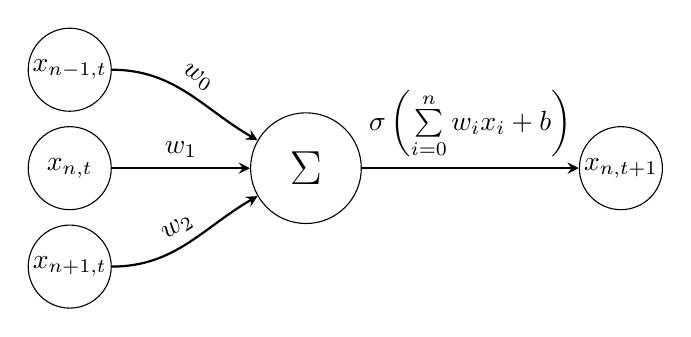
\begin{tikzpicture}
	\node[draw,circle,minimum size=40pt,inner sep=0pt] (x) at (0,0) {\LARGE $\Sigma$};
	
	\node[inputNode,minimum size=30pt] (x1) at (-3, 1.25) {$x_{n-1,t}$};
	\node[inputNode,minimum size=30pt] (x2) at (-3, 0) {$x_{n,t}$};
	\node[inputNode,minimum size=30pt] (x3) at (-3, -1.25) {$x_{n+1,t}$};
	\node[inputNode,minimum size=30pt] (x4) at (4, 0) {$x_{n,t+1}$};
	
	\draw[stateTransition] (x1) to[out=0,in=150] node [midway, sloped, above] {$w_0$} (x);
	\draw[stateTransition] (x2) to[out=0,in=180] node [midway, sloped, above] {$w_1$} (x);
	\draw[stateTransition] (x3) to[out=0,in=210] node [midway, sloped, above] {$w_2$} (x);
	\draw[stateTransition] (x) to[out=0,in=180] node [midway, sloped, above] {$\sigma \left( \sum\limits_{i=0}^{n}{w_ix_i} + b \right)$} (x4);
	\end{tikzpicture}
	
	\label{fig:mst_neuronalnetworkdemo}
	\caption{Einige Beispiele von Kurven die Mittels Hermite-Polynom erzeugt wurden.}
\end{figure}

Zusätzlich können einigen Restriktionen eingebaut werden:
\begin{itemize}
	\item {\textbf{$\sigma$:} Als Aktivierungsfunktion wird eine lineare Funktion gewählt.}
	\item {\textbf{$b$: } Die Bias-Variable wird auf 0 gesetzt und während dem Training nicht verändert, es ist zu erwarten, dass $b=0$ sein muss!}
	\item {\textbf{$w_{0,1,2}$: } Die Parameter für das Gewicht werden trainiert, es könnte hier noch noch $w_0 = w_2$ in Erwägung gezogen werden, um die Symetrie auszunutzen.}
\end{itemize}
Das Netz hat somit 3 Parameter $w_0, w_1, w_2$ welche erlernt werden müssen. Aus der mathematischen Herleitung ist zu erwarten, dass der Gewichtsvektor $w_{0,1,2}$ die Lösungsform $w = \xi \cdot (1, -2, 1)$ annimmt. $\xi$ ist an dieser Stelle ein Platzhalter für $\xi = \frac{\kappa}{h^{2}}$ welche einfach zusammen gefasst werden können.

\subsection{Trainingsdaten und 'faire' Kurven}
Mit dem Verständnis für neuronale Netzwerke müssen nun die Daten erschaffen werden um das Netzwerk zu trainieren. Als Grundlage zum erlernen der Wärmeleitungsgleichung wird logischerweise die selbe Funktion verwendet um den Input $I_{t}$ und Output $O_{t}$ zu generieren. Da das Netzwerk dazu neigt 'Trivialitäten' zu lernen, muss bei der Datengenerierung geachtet werden, dass kein Muster in den Daten vorhanden ist, welche nicht mit der Wärmeleitungsgleichung zusammenhängen. Beispielsweise kann davon ausgegangen werden, dass wenn nur monoton steigende Funktionen im Training verwendet werden, das Netzwerk vermutlich Mühe habt eine akkurate Vorhergsage für eine monoton fallende Funktion zu treffen. Aus diesem Grunde werden 'faire' Kurven verwendet, welche unterschiedlichste Verschiebungen, Krümmungen und Wendepunkte aufweisen. So kann sichergestellt werden, dass das Netz als einziges Muster die tatsächliche Wärmeleitungsgleichung erlernt. Als besonders hilfreich haben sich hier die Hermite-Polynome erwiesen.

\begin{align}
H_{n}(x) &=(-1)^{n}e^{x^{2}}{\frac {d^{n}}{d x^{n}}}e^{-x^{2}} \\
H_{n}(x) &=(-1)^{n}\sum _{k_{1}+2k_{2}=n}{\frac {n!}{k_{1}!k_{2}!}}(-1)^{k_{1}+k_{2}}(2x)^{k_{1}}
\end{align}

Die ersten 5 Hermite Polynome sind in einfacher Schreibweise folgende:

\begin{align}
H_{0}(x) &= 1\\
H_{1}(x) &= 2x\\
H_{2}(x) &= 4x^{2}-2\\
H_{3}(x) &= 8x^{3}-12x\\
H_{4}(x) &= 16x^{4}-48x^{2}-12
\end{align}

Zur Generierung der Daten wurde ein Vektor $v=(H_0, \dots ,H_9)$ gwählt. Jedes Element in diesem Vektor representiert ein Hermite Polynom n-ten Grades. Dies wird benötigt um kleine Hermite Polynome zu verwenden und mittels Linearkombination verscheidene Kurven zu generieren. Es soll vermieden werden, dass zu grosse Werte entstehen oder zu extreme Krümmunen entstehen daher wurde auf ein Grad über 10 abgesehen. Das Polynom 10ten Grades hat als dominanten Faktor $1024 \cdot x^{10}$ was zeigt wie schnell die Kurven gegen den Rand ansteigen, dies wird in Abbildung \ref{fig:mst_hermite_big} nocheinmal verdeutlicht.

\begin{figure}[h]
	\centering
	\begin{tabular}{cc}
		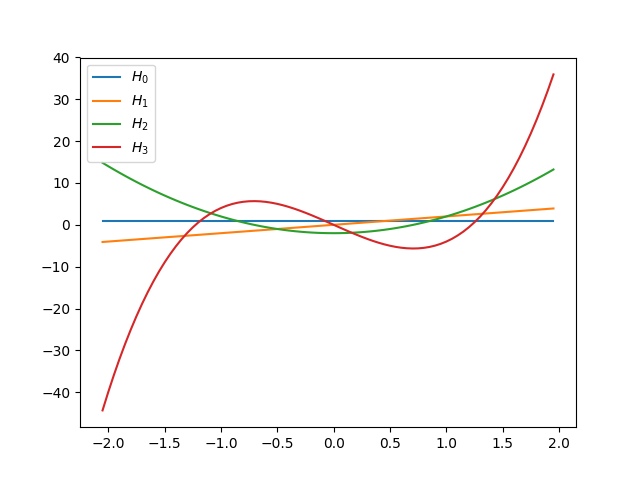
\includegraphics[scale=0.40]{learning/img/hermite_small.png} &
		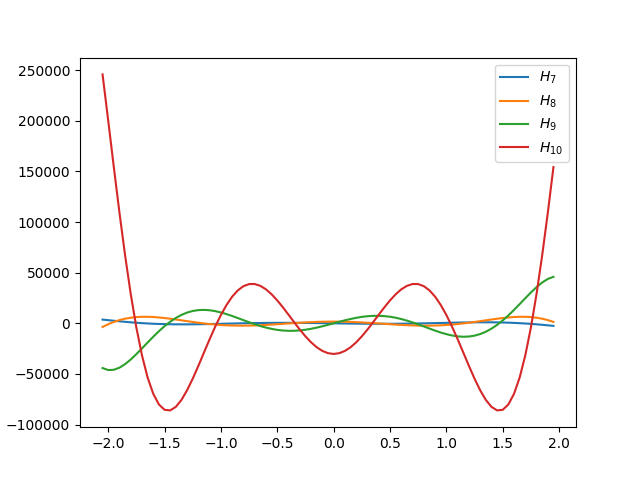
\includegraphics[scale=0.40]{learning/img/hermite_big.png} 
	\end{tabular}
	\label{fig:mst_hermite_big}
	\caption{\textbf{Links:} Die Hermite Polynome 0-ten bis 3-ten Grades \textbf{Rechts:} $H_{10}$ soll verdeutlichen wie extrem die Entwicklung zu den Rändern sich entwickelt.}
\end{figure}

\begin{figure}[h]
	\centering
	\begin{tabular}{ccc}
		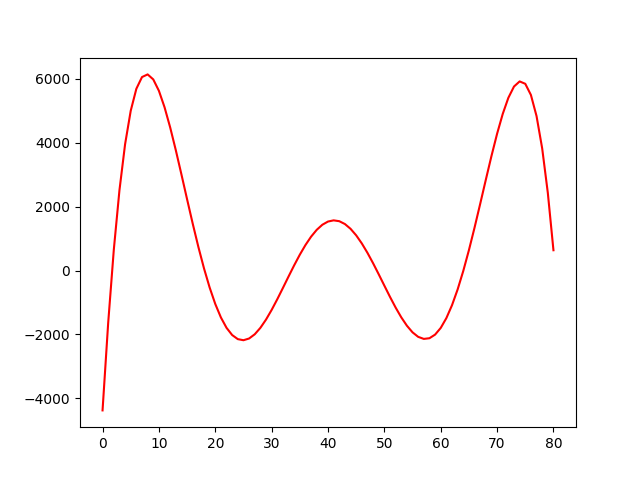
\includegraphics[scale=0.25]{learning/img/curves/wave0.png} &
		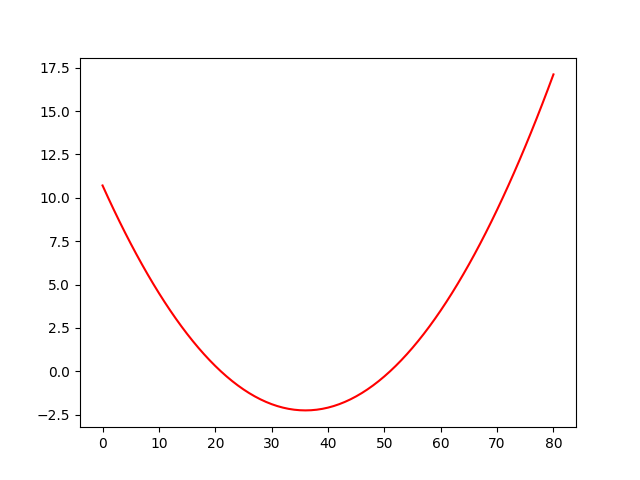
\includegraphics[scale=0.25]{learning/img/curves/wave1.png} &
		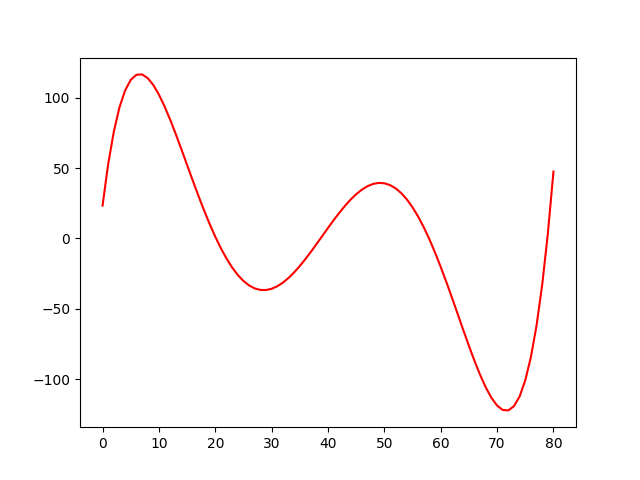
\includegraphics[scale=0.25]{learning/img/curves/wave2.png} \\
		
		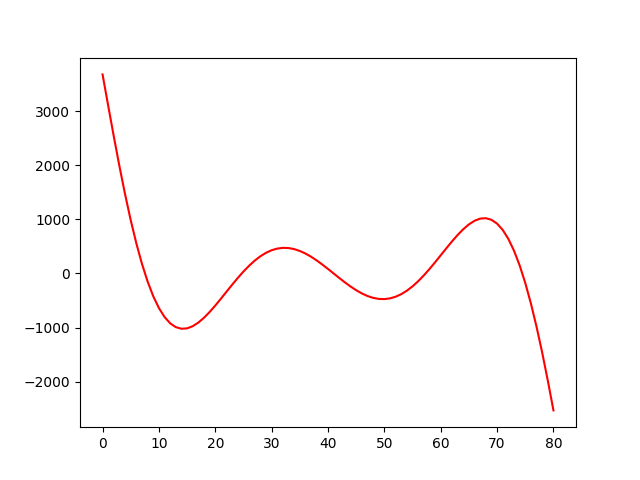
\includegraphics[scale=0.25]{learning/img/curves/wave8.png} &
		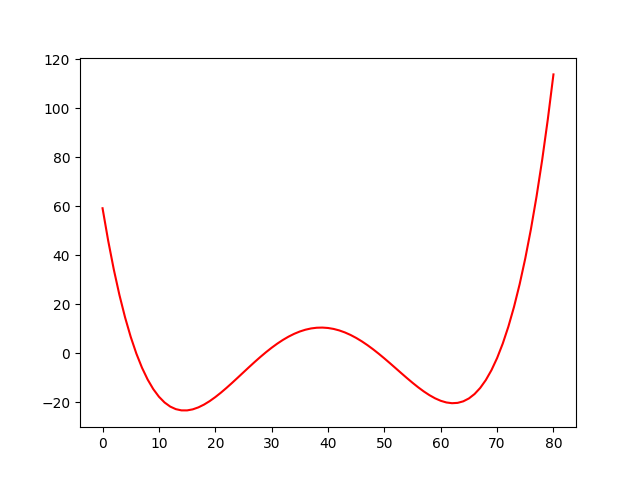
\includegraphics[scale=0.25]{learning/img/curves/wave4.png} &
		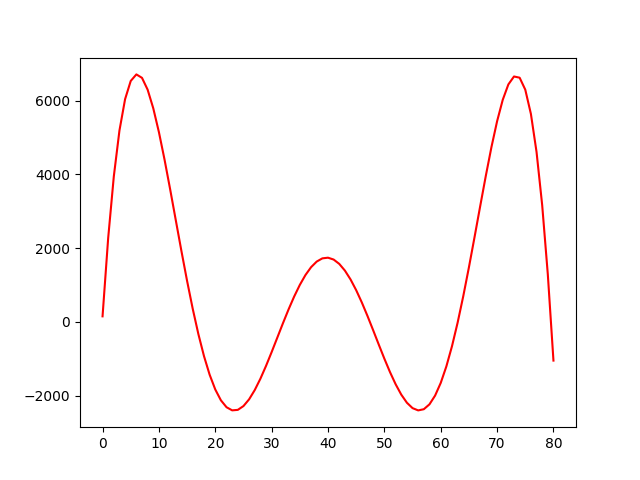
\includegraphics[scale=0.25]{learning/img/curves/wave3.png}
	\end{tabular}
	\label{fig:mst_hermiteexample}
	\caption{Einige Beispiele von Kurven die Mittels Hermite-Polynom erzeugt wurden.}
\end{figure}

Aus den generierten Kurven werden mithilfe eines ODE-Solvers die Input und Output Daten erzeugt. Die Kurven werden diskretisiert und aus Form-Gründen in die Vektoren $I_n$ und $O_n$ aufgeteilt. Die Diskretisierung erfolt auf dem Interval [-2.05, 2) mit einem Abstand von 0.05, dies resultiert in 80 Punkten, welche zu Input Vektoren konvertiert werden. Es werden pro Kurve mehrere Vektorpaare gebildet um die Daten so gut wie möglich auszunutzen. Mihilfe dieser Daten wird nun das Neuronale Netzwerk trainiert.

\subsection{Resultate}
Nach zahlreichen Trainingsanläufen mit unzähligen Iterationen kann festgehalten werden, dass die mathematische Herleitung genau dem erlernten des Neuronalen Netzwerks entspricht (vgl. Tabelle \ref{tbl:result_heat}) Das Tabelle enthält nur ein Beispiel welches aus dem Training hergeleitet werden konnte. Die Resutlate sind nicht deterministisch, da die Generierung der Daten randomisiert stattgefunden hat. Wichtig ist aber, dass die Lösungsform ($w = \xi \cdot (1, -2, 1)$) stets erfüllt wurde und die L1-Norm von $w$ jederzeit sehr nahe bei $1$ war.

\begin{table}[h]
	\centering
	\def\arraystretch{1.1}
	\begin{tabular}{l|c|c}
		Parameter & Erwartung & Experiment \\
		\hline
		$w$ & $\xi \cdot \begin{bmatrix} 1 \\ -2 \\ 1 \end{bmatrix}$ & $\begin{bmatrix} 0.36 \\ -0.73 \\ 0.37 \end{bmatrix}$ \\
		$\|w\|_{1}$ & 1 & $\sim 1$ \\
		$b$ & 0 & 0 \\
	\end{tabular}
	\label{tbl:result_heat}
	\caption{Resultate der erlernten Wärmeleitungsgleichung.}
\end{table}

Es wurde mit einem einfachen Experiment gezeigt, dass das Lernverhalten des Neuronalen Netzwerkes anhand eines einfachen Beispiels verstanden werden kann und durchaus durchschaubar ist. Das Problem dieses Beispiels ist jedoch, dass ein KNN nicht wirklich benötigt wird, da im Grunde die Lösung numerisch einfach bestimmt werden kann.


%
% burgerintro.tex
%
% (c) 2018 Prof Dr Andreas Müller, Hochschule Rapperswil
%
\section{Die Gleichung von Burgers}
Die Gleichung von Burgers ist ein prototypisches Beispiel einer nichtlinearen
partiellen Differentialgleichung, an dem sich viele für nichtlineare
Differentialgleichungen typische Phänomene in einer einfachen Situation
studieren lassen.
Zum Beispiel tritt bei einigen numerischen Lösungsverfahren für die
Gleichung von Burgers häufig eine Instabilität auf, die man 
Computational Mode nennt.
Natürlich sind Tricks entwickelt worden, mit diesem Problem fertig
zu werden.
Der zuvor für die Wärmeleitungsgleichung untersuchte Ansatz, ein
Lösungsverfahren mit Hilfe von Machine Learning zu konstruieren, birgt
das Potential, den Computational Mode von Anfang an zu vermeiden.
Das Verfahren kann nur lernen, was auch in den Trainingsdaten
erkennbar ist, und wir können sicherstellen, dass die Trainingsdaten
keine Lösungen enthalten, die Anzeichen des Computational Mode beinhalten.

In diesem Abschnitt sammeln wir ein paar Fakten über die Gleichung 
von Burgers und den Computational mode.
In einem späteren Abschnitt werden wir diese Informationen dazu
verwenden, um Trainingsdaten zu erzeugen.

\subsection{Nichtlineare Transportgleichung\label{subsection:nichtlineare}}
Die Gleichung von Burgers in der Form
\begin{equation}
\frac{\partial u}{\partial t} + u\frac{\partial u}{\partial x}=0
\qquad\text{mit Anfangsbedingung}\qquad
u(0,x) = u_0(x)
\label{burgers:transport}
\end{equation}
modelliert ein nichtlneares Transportproblem.
Die Gleichung~\eqref{burgers:transport} ist eine quasilineare partielle
Differentialgleichung erster Ordnung, die mit der Methode der
Charakteristiken \cite{burgers:pde} gelöst werden kann.
Die Charakteristiken-Gleichungen sind
\begin{align*}
t'(s)&=1
\\ 
x'(s)&=u
\\
u'(s)&=0
\end{align*}
Aus der ersten Gleichung leitet man ab, tdass $s=t$.
Die dritte Gleichung besagt, dass $u$ entlang einer Charakteristik konstant
ist, also $u(s)=u_0$.
Die zweite Gleichung besagt dann, dass die im Punkt $(0,x_0,u_0(x_0))$
beginnende Charakteristik eine Gerade mit $x(t)=x_0 + u_0(x_0)t$ ist.

\begin{figure}
\centering
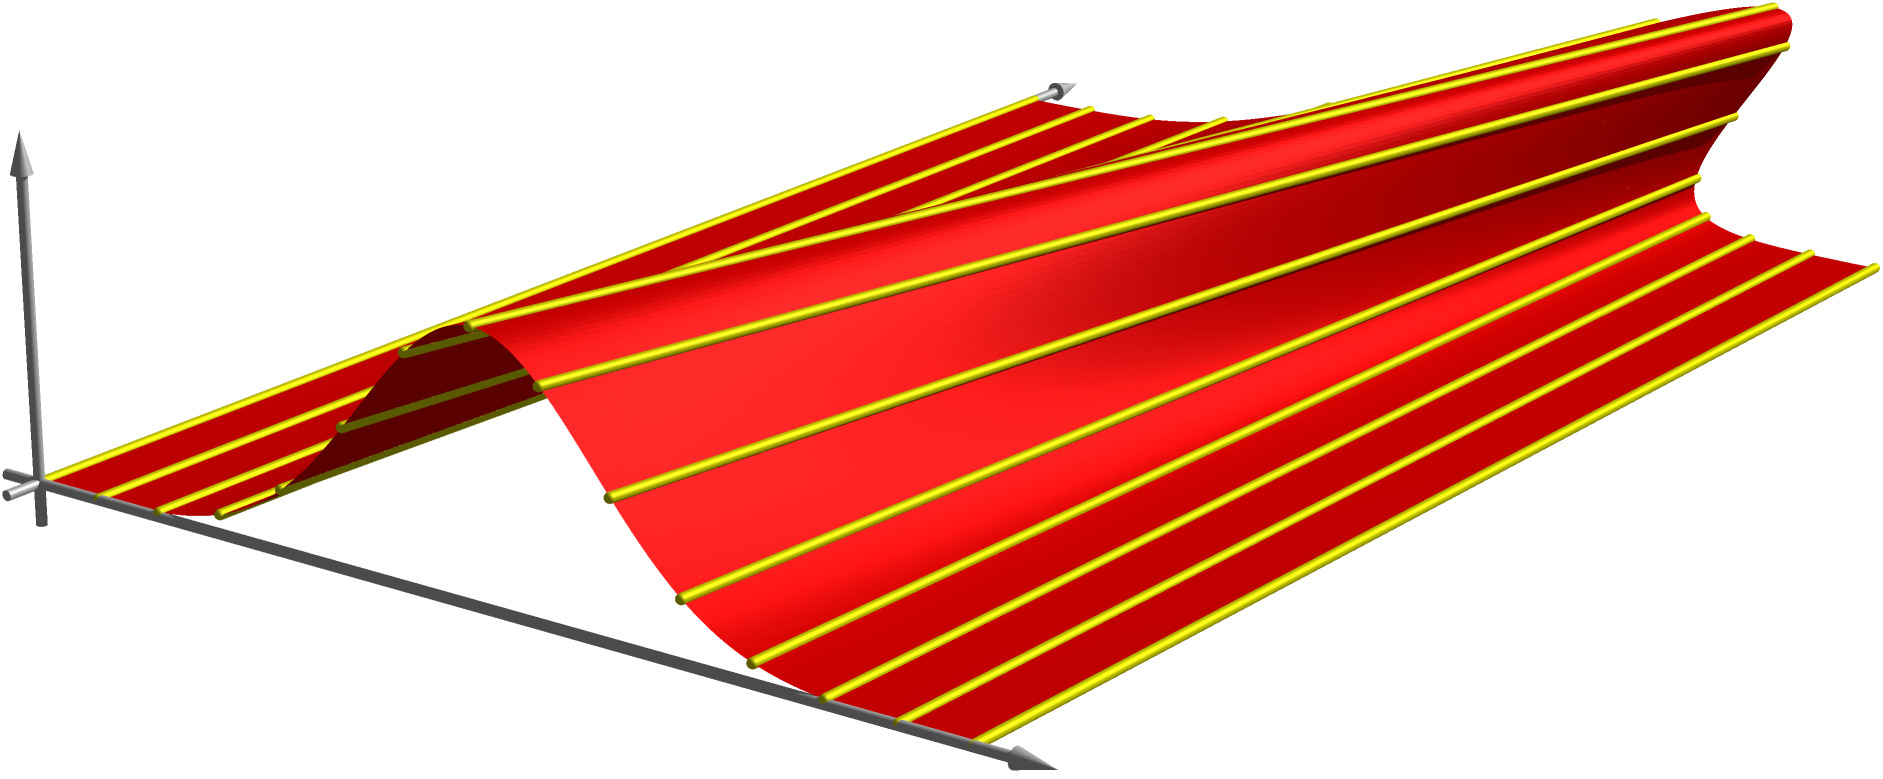
\includegraphics[width=\hsize]{learning/welle.jpg}
\caption{Lösung der Gleichung von Burgers mit Hilfe der Methode
der Charakteristiken.
Die Lösungsfläche ist darstellbar als eine Schar von Geraden (gelb).
\label{burgers:charloesung}}
\end{figure}
Die Abbildung~\ref{burgers:charloesung} 
zeigt eine Lösung mit einer Gauss-Verteilung als Anfangsbedingung.
Es ist offensichtlich, dass die gezeigte Fläche früher oder später nicht
mehr Graph einer Funktion $u(x,y)$ sein kann.
Es entwickelt sich eine Sprungstelle, die Gleichung von Burgers ist
ein Modell für eine Schockwelle.
Man kann insbesondere nicht erwarten, dass die Gleichung von Burgers
für beliebige Zeiten $t$ eine glatte Lösung hat, selbst wenn die
Anfangsbedingungen glatt waren.
Man muss sich mit einer schwachen Lösung begnügen.
Dies hat sowohl auf numerische Lösungsverfahren Auswirkungen wie auch
auf das Problem, Trainingsdaten für auf Machine Learning basierenden
Lösungsalgorithmus zu erzeugen.

\subsection{Erhaltungssatz\label{subsection:erhaltungssatz}}
Die Gleichung von Burgers kann man auch in der Form
\begin{equation}
\frac{\partial u}{\partial t}
+
\frac{\partial}{\partial x} \frac{u^2}{2}
=
0
\label{burgers:erhaltungssatz}
\end{equation}
formulieren.
Dies ist ein Spezialfall der allgemeineren Gleichung
\begin{equation}
\frac{\partial u}{\partial t}
+
\frac{\partial }{\partial x} F(u)
=
0
\label{burgers:conservationlaw}
\end{equation}
mit $F(u)=\frac12u^2$.
Man nennt 
\eqref{burgers:conservationlaw}
einen Erhaltungssatz.
Diese Betrachtungsweise erlaubt, die Bewegung von Sprungstellen besser
zu verstehen.

Die Differentialgleichung~\eqref{burgers:conservationlaw} kann auch
in der Form
\[
\frac{\partial u}{\partial t}
+
\frac{\partial }{\partial x} F(u)
=
\begin{pmatrix}
\frac{\partial}{\partial t}
\\
\frac{\partial}{\partial x}
\end{pmatrix}
\begin{pmatrix}t\\F(u)\end{pmatrix}
=
\nabla\cdot 
\begin{pmatrix}t\\F(u)\end{pmatrix}
=0
\]
schreiben.
Darauf ist aber der Satz \ref{skript:wegunabhaengigkeit} anwendbar.
Er besagt, dass Integrale
\begin{align}
\oint_\gamma(
F(u)\,dt
-
u\,dx
)
&=
\int_D \frac{\partial u}{\partial t}+\frac{\partial}{\partial x}F(u)\,dx\,dy
=
0
\label{burgers:integral}
\end{align}
über geschlossene Wege $\gamma$ verschwinden.

\subsection{Hugoniot-Rankine-Bedingungen\label{subsection:hugnoniot}}
\begin{figure}
\centering
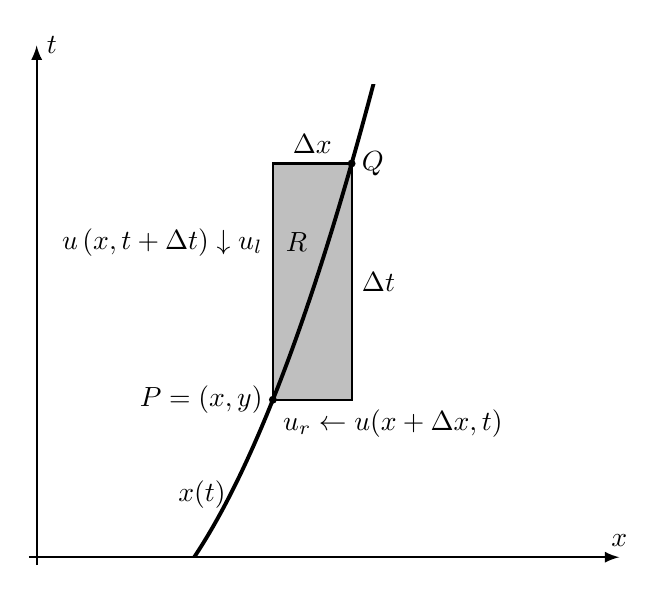
\begin{tikzpicture}[>=latex,thick]
\fill[color=gray!50] (3,2)--(4,2)--(4,5)--(3,5)--cycle;
\node at (3.3,4.0) {$R$};
\draw[->] (-0.1,0)--(7.4,0) coordinate[label={$x$}];
\draw[->] (0,-0.1)--(0,6.5) coordinate[label={right:$t$}];
\fill (3,2) circle[radius=0.05];
\node at (3,2) [left] {$P=(x,y)$};
\fill (4,5) circle[radius=0.05];
\node at (4,5) [right] {$Q$};
\draw (3,2)--(4,2)--(4,5)--(3,5)--cycle;
\node at (3.5,5) [above] {$\Delta x$};
\node at (4,3.5) [right] {$\Delta t$};
\begin{scope}
\clip (0,0) rectangle (7,6.0);
\draw[line width=1.4pt] plot[domain=2:5,samples=100] ({\x},{0.5*\x*\x -0.5*(\x)-1});
\end{scope}
\node at (3,4) [left] {$\begin{matrix}u(x,t+\Delta t)\\\downarrow\\u_l\end{matrix}$};
\node at (3,2) [below right] {$u_r\leftarrow u(x+\Delta x,t)$};
\node at (2.1,0.8) {$x(t)$};
\end{tikzpicture}
\caption{Herleitung der Hugoniot-Rankine-Bedingung für die Bewegung einer
Sprungstelle der Lösung eines Erhaltungssatzes.
\label{burgers:hugoniot}}
\end{figure}
In Abschnitt~\ref{subsection:nichtlineare} haben wir gesehen, dass Lösungen
der Gleichung von Burgers Sprungstellen entwickeln.
Die Formulierung als Erhaltungssatz in
Abschnitt~\ref{subsection:erhaltungssatz} 
soll uns jetzt erlauben, die Bewegung solcher Sprungstellen zu beschreiben.

Sie also $u(t,x)$ eine Lösung fast überall der Gleichung von Burgers mit
einer Sprungstelle, die sich entlangt der Kurve $x(t)$ bewegt.
Dazu berechnen wir das Wegintegral \eqref{burgers:integral} über den Rand
des Rechtecks mit den Ecken $(x,y)$ und $(x+\Delta x, y+\Delta y)$.
Wir benötigen die Grenzwerte
\[
\begin{aligned}
u_l &= \lim_{\Delta t\to 0+} u(t+\Delta t,x)
&&\text{und}&
u_r &= \lim_{\Delta x\to 0+} u(t,x+\Delta x).
\end{aligned}
\]
Damit können wir das Wegintegral approximieren als
\begin{align}
\int_{\partial R}(u\,dx -F(u)\,dt)
&=
0
\notag
\\
u(t+\Delta t,x)
\Delta x
-
F(u(t+\Delta t,x))
\Delta t
&=
u(t,x+\Delta x) \Delta x
-
F(u(t,x+\Delta x)) \Delta t
\notag
\\
\Delta x
(
u(t+\Delta t,x)
-
u(t,x+\Delta x)
)
&=
\Delta t
(F(u(t+\Delta t,x))
-
F(u(t,x+\Delta x))
)
\notag
\\
\intertext{Oder nach Grenzübergang $\Delta t\to 0$ und $\Delta x\to 0$}
\dot x(t)\, (u_l-u_r) &= F(u_l) - F(u_r).
\label{burgers:hugoniot-rankine}
\end{align}
Die Geschwindigkeit, mit der sich die Sprungstelle bewegt, hängt also 
von den Werten von $u(t,x)$ auf beiden Seiten der Sprungstelle ab.
Dies sind die {\em Hugoniot-Rankine-Bedingungen}.
Wir werden sie Abschnitt~\ref{burgers:training} verwenden, um Trainingsdaten
für Sprungstellen der Lösung zu erzeugen.
\index{Hugoniot-Rankine-Bedingungen}
\index{Rankine-Hugoniot-Bedingungen}

Im Fall der Gleichung von Burgers ist $F(u)=\frac12u^2$.
Die Hugoniot-Rankine-Bedingung wird dann zu
\begin{equation}
\dot x(t)\, (u_l-u_r) = \frac12 (u_l^2-u_r^2)
\qquad\Rightarrow\qquad
\dot x(t)
=
\frac12 (u_l+u_r).
\end{equation}
Eine Sprungstelle der Gleichung von Burgers bewegt sich also immer
mit der Geschwindigkeit, die dem Mittelwert der $u$-Werte auf
beiden Seiten der Sprungstelle entspricht.

\subsection{Numerische Lösungen und Computational mode}
Bei der numerischen Lösung der Gleichung von Burgers tritt erschwehrend ein
Computational Mode auf.
Ziel dieses Abschnittes ist, die Herkunft des Computational Mode zu erklären
und an einem numerischen Experiment zu illustrieren, wie er auch bei
der Gleichung von Burgers zu Instabilität bei der numerischen
Lösung führen kann.

\subsubsection{Ein einfacheres Beispiel}
Wir betrachten die gewöhnliche Differentialgleichung
\begin{equation}
\frac{du}{dx}=0.
\label{burgers:konstant}
\end{equation}
Die einzigen Lösungen dieser Differentialgleichungen sind die konstanten
Funktionen.
Wir würden also erwarten, dass auch ein numerisches Verfahren nur
die konstanten Funktionen als Lösungen hervorbringen würde.

Wir beginnen mit einer Diskretisierung $x_i=ih$, $i\in\mathbb N$, und
versuchen eine Lösung $u_i= u(x_i)$ zu konstruieren.
Die Ableitung wird durch Differenzenquotienten approximiert, dies
führt auf die Gleichungen
\begin{equation}
0
=
\frac{du(x_i)}{dx}
=
\frac{u_{i+1}-u_{i}}{x_{i+1}-x_{i}} = \frac{u_{i+1}-u_i}{h},
\label{burgers:diffquot}
\end{equation}
was gleichbedeutend ist mit der Rekursionsgleichung
\[
u_{i+1} = u_{i}.
\]
Diese besagt natürlich nichts anderes als dass wie erwartet
die Lösungsfunktion konstant sein muss.

Das Problem dieses Beispiel ist jedoch, dass der Differenzenquotient
\eqref{burgers:diffquot} gar nicht repräsentativ ist für eine Ableitung
an der Stelle $x_i$, sondern eher für $u'(x_i+\frac12h)$.
Ein symmetrischer Differenzenquotient 
\[
u'(x_i)
\simeq
\frac{u_{i+1}-u_{i-1}}{x_{i+1}-x_{i-1}}=\frac{u_{i+1}-u_{i-1}}{2h}=0
\]
ist zutreffender, führt aber auf die Rekursionsgleichung
\[
u_{i+1}=u_{i-1}.
\]
Diese hat zwei linear unabhängige Lösungen, die Gleichungen besagen
nämlich nur, dass alle geraden Werte $u_{2i}=u_0$ und alle ungeraden
$u_{2i+1}=u_1$ sind, diese beiden Werte können aber durchaus verschieden
sein.
Der Versuch, den Differenzenquotienten genauer wiederzugeben hat 
zusätzliche numerische Lösungen hervorgebracht, die nichts mit Lösungen
der Differentialgleichung zu tun haben.

\subsubsection{Differentialgleichung für die Exponentialfunktion}
Das Beispiel~\eqref{burgers:konstant} war insofern künstlich, als auf der
rechten Seite die Werte von $u$ gar nicht gebraucht wurden und daher das
Argument, der Differenzenquotient~\eqref{burges:diffquote} können nicht
mit der rechten Seite verglichen werde, nicht wirklich stichhaltig ist.
Dies ändert sich mit der Gleichung
\begin{equation}
\frac{du}{dx} = -u.
\label{burgers:expo}
\end{equation}
Der Differenzenquotient auf der linken Seite wird hier mit einem
Funktionswert auf der rechten Seite verglichen. 
Der einfachste Ansatz ist wieder
\[
\frac{u_{i+1}-u_i}{x_{i+1}-x_{i}}
=
\frac{u_{i+1}-u_i}{h} = -u(x_i) = -u_i
\qquad\Rightarrow\qquad
u_{i+1} = u_i-hu_i=(1-h)u_i,
\]
mit der eindeutigen Lösung
\[
u_i = (1-h)^iu_0.
\]
Um $u(x)$ mit einer Diskretisierung mit $n$ Schritten zu berechnen,
muss die Schrittweite $h=x/n$ verwendet werden, so dass wir für
\[
u(x) \simeq \biggl(1-\frac{x}{n}\biggr)^n u_0
\]
erhalten.
Im Grenzwert $n\to\infty$ ist
\[
u(x) = \lim_{n\to\infty} \biggl(1-\frac{x}{n}\biggr)^n u_0 = u_0e^{-x}
\]
die korrekte Lösung der ursprünglichen Differentialgleichung.

Das eben diskutierte Verfahren ist natürlich das {\em Euler-Verfahren}.
\index{Euler-Verfahren}
Seine Genauigkeit bei grosser Schrittweite $h$ ist sehr beschränkt,
was unter anderem auch damit zu tun hat, dass der Differenzenquotient
nicht repräsentativ ist für die Ableitung an der Stelle $x_i$.
Wir versuchen daher wieder einen symmetrischen Differenzenquotienten
und erhalten
\begin{equation}
\frac{u_{i+1}-u_{i-1}}{x_{i+1}-x_{i-1}}
=
\frac{u_{i+1}-u_{i-1}}{2h}
=
-u_{i}
\qquad\Rightarrow\quad
u_{i+1}=u_{i-1}-2hu_{i}
\label{burgers:diffgl}
\end{equation}
Wir lösen die lineare Differenzengleichung \eqref{burgers:diffgl} mit einem
Potenzansatz $u_i=\lambda^i$, dies ergibt die charakteristische Gleichung
\[
\lambda^2+2h\lambda-1=0,
\]
die die Lösungen
\[
\lambda = -h\pm\sqrt{h^2+1}.
\]
Die Ableitung der Wurzelfunktion an der Stelle $1$ ist $\frac12$, so dass
$\lambda$ approximiert werden kann durch
\[
\lambda = \pm(1+\frac12h^2+\dots)- h
=
\begin{cases}
\phantom{-}1-h-\frac12h^2+\dots&=\lambda_+\\
-1-h-\frac12h^2+\dots&=\lambda_-
\end{cases}
\]
Die erste Lösung $\lambda_+$ ist positiv und $\lambda_+<1$, sie führt auf
die gleiche Lösung, die wir schon beim Euler-Verfahren gefunden haben.
\begin{figure}
\centering
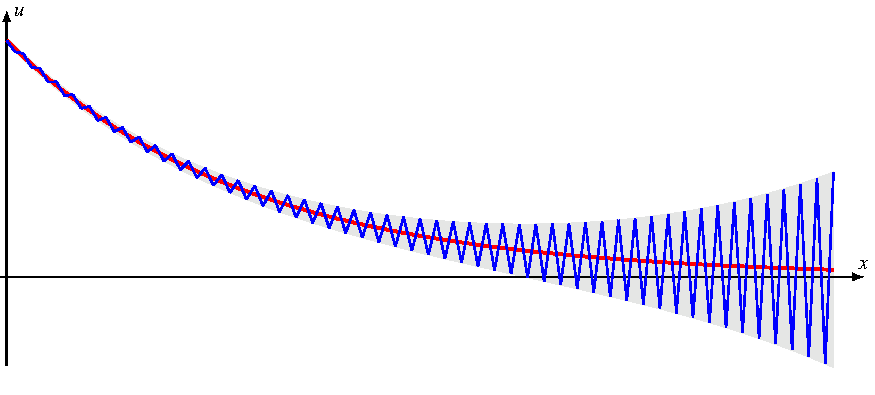
\includegraphics{learning/compmod.pdf}
\caption{Exakte Lösung (rot) und numerische Lösung (blau)
der Differentialgleichung
\eqref{burgers:expo}
unter Verwendung symmetrischer Differenzenquotienten.
Der Computational Mode äussert sich im exponentiellen Anwachsen
alternierender Fehler mit grösser werdendem $x$.
\label{burgers:compmod}}
\end{figure}

Die zweite Lösung $\lambda_-$ ist negativ und $|\lambda_-|>1$ für $h$
klein genug.
Die Gleichung~\ref{burgers:diffgl} hat also eine zusätzliche Lösung
$u_i=u_0\lambda_-^i$ mit alterniernden Vorzeichen, die sehr schnell anwächst.
Wir können wie bei $\lambda_+$ auch den Grenzwert für beliebig feine
Diskretisierung bestimmen.
Da das Vorzeichen dieser Lösung mit jedem Schritt wechselt, untersuchen
wir nur die geraden Schritte.
Wir nehmen wieder $h=x/2n$ und berechnen den Grenzwert
\[
\lim_{n\to\infty}
u_0
\biggl(
1+\frac{x}{2n}+\dots
\biggr)^{2n}
=
u_0e^x.
\]
Die Lösung wächst also exponentiell schnell an.

Die Lösung der Differentialgleichung ist eine Linearkombination
\[
u_i = a_+\lambda_+^i + a_-\lambda_-^i,
\]
deren Koeffizienten aus Anfangswerten bestimmt werden müssen.
Für fast alle Anfangswerte ist unvermeidbar, dass sich der
Koeffizient $a_-$ als von $0$ verschieden herausstellt, auch
wenn er sehr klein ist.
Weil $\lambda_-^i$ exponentiell schnell anwächst wird der Summand
$a_-\lambda_-^i$ immer früher oder später die numersiche Lösung dominieren,
wie dies auch in Abbildung~\ref{burgers:compmod} dargestellt ist.

Diese Lösung ist einzig entstanden durch den Versuch, mit Hilfe zusätzlicher
Funktionswerte das numerische Verfahren zu verbessern.
Dabei ist die Ordnung der Differenzengleichung grösser geworden und damit
sind neue Lösungen entstanden.

\subsubsection{Gleichung von Burgers und Computational Mode}
\begin{figure}
\centering
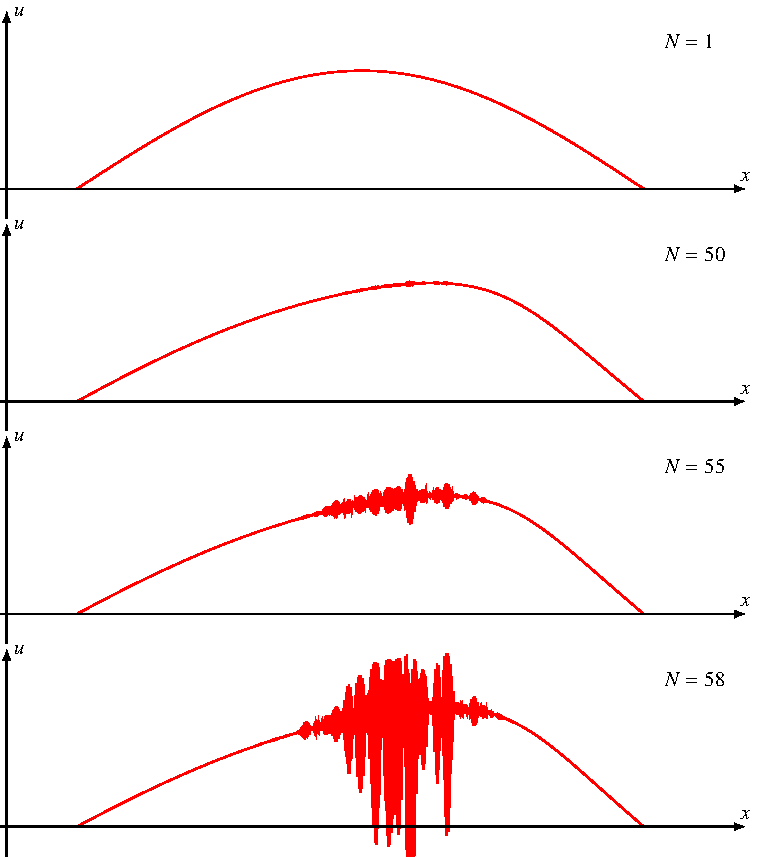
\includegraphics{learning/burgerwave.pdf}
\caption{Entwicklung des Computational Mode in einer Simulation
der Differenzengleichung \eqref{burgers:diffgleichung}.
Im obersten Graphen sieht man die Anfangsbedingung, die Funktion $sin x$
zwischen $0$ und $2\pi$.
Bei Iteration $N=50$ kann man bereits erkennen, wie sich der Computational
Mode auszuwirken beginnt, die nachfolgend gezeigten Iterationen sind
unbrauchbar.
\label{burgers:burgerwave}}
\end{figure}
Das Problem des Computational Mode tritt auch bei der Gleichung von Burgers
auf.
Wir verwenden eine zweidimensionale Diskretisation $(t_i, x_j)$ mit
Schrittweite $h$.
Die asymmetrischen Differenzenquotienten
\[
\frac{\partial u(t_i,x_j)}{\partial t}
\simeq
\frac{u_{i+1,j} - u_{i,j}}{2h}
\qquad\text{und}\qquad
\frac{\partial u(t_i, x_j)}{\partial x}
\simeq
\frac{u_{i,j+1} - u_{i,j}}{2h}
\]
sind nicht wirklich repräsentativ für den Gitterpunkt $(i,j)$.
In die Gleichung geht zusätzlich zu den Ableitungen auch noch der
Funktionswert $u_{ij}$, was unterstreicht, dass wir die Ableitungen
möglichst genau an der Stelle $(i,j)$ bestimmen können müssen.

Die besser geeigneten symmetrischen Differenzenquotienten 
\[
\frac{\partial u(t_i,x_j)}{\partial t}
\simeq
\frac{u_{i+1,j} - u_{i-1,j}}{2h}
\qquad\text{und}\qquad
\frac{\partial u(t_i, x_j)}{\partial x}
\simeq
\frac{u_{i,j+1} - u_{i,j-1}}{2h}
\]
führen auf die nichtlineare Differenzengleichung
\begin{equation}
u_{i+1,j}
= 
u_{i-1,j}
+
h
u_{ij}\frac{u_{i,j+1}-u_{i,j-1}}{h}
=
u_{i-1,j}
+
u_{ij}(u_{i,j+1}-u_{i,j-1}),
\label{burgers:diffgleichung}
\end{equation}
die ebenfalls mindestens zweiter Ordnung ist.
Auch sie zeigt den Computational Mode, wie man zum Beispiel auch
in numerischen Experimenten sehen kann (Abbildung~\ref{burgers:burgerwave}).






%
% burgertraining.tex -- Trainingsdaten für Burgers Gleichung
%
% (c) 2018 Prof Dr Andreas Müller, Hochschule Rapperswil
%
\subsection{Trainingsdaten für die Gleichung von Burgers}
Damit die Gleichung von Burgers mit einem Machine-Learning-Ansatz gelöst
werden kann, müssen geeignete Trainingsdaten bereitgestellt werden.

\subsubsection{Lösung mit Charakteristiken}

\subsubsection{Sprungstellen}



\printbibliography[heading=subbibliography]
\end{refsection}
